\subsection{CNN}

The task of \textit{finding the coordinates of the bubbles} can be read as \textit{for each pixel, check if it is the center of a bubble}.
The task of looking for the same thing across all pixels of an image is the foundation of image convolution and convolutional layers in neural network.
As such, a SAME CONV neural layer was proposed, with a kernel size big enough for containing a full bubble.
The CNN would transform the input image into a binary image, where ``on'' pixels would represent bubble centers.

\subsubsection{Algorithm}

\begin{itemize}
	\itemsep 0em
	\item Initially, the single-layer CNN evaluates the image, to find centroids of the bubbles;
	\item At a second stage, a loop would collect all the ``on'' pixels of the image into a list of coordinates.
\end{itemize}

\subsubsection{Evaluation}

Initially, only a feasibility study was performed: the CNN was trained with just a single epoch of 8 images, to evaluate if the inference speed was good enough to justify a longer training.
The result shown in figure~\ref{fig:locate:cnn} is promising for the little training performed, but it clearly needs more refinement.

Most importantly, the speed was much greater than the previous ones, at 55 FPS, but still far from the target.
As such, further approaches were evaluated before performing a deeper training, to investigate if a greater speed was achievable.

\begin{figure}
	\centerline{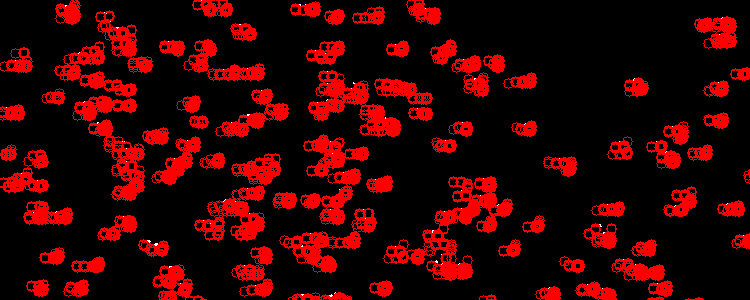
\includegraphics[width=\locateimgsize]{images/locate/cnn.png}}
	\caption{\centering The CNN's result}
	\label{fig:locate:cnn}
\end{figure}
